\section{সত্যক সারণি, সমীকরণ ও সার্কিট}
একই যৌক্তিক কাজকে কথায়, সত্যক সারণিতে, বুলিয়ান সমীকরণে এবং সার্কিটে প্রকাশ করা যায়। কথার শর্তকে আগে ইনপুটের ০ ও ১ দিয়ে নির্দিষ্ট করলে পরের ধাপগুলো সহজ হয়।

\subsection{সারণি থেকে সমীকরণ: SOP ও POS}
যে সারিতে আউটপুট ১, সেই সারির জন্য প্রতিটি চলক নিয়ে একটি AND পদ তৈরি করো। ইনপুট ১ হলে সরাসরি চলক, ০ হলে পূরক। পদগুলো OR করলে \textbf{গুণফলের যোগফল} বা SOP পাওয়া যায়। সব চলক থাকা এমন একটি পদকে \textbf{মিনটার্ম} বলে।

যে সারিতে আউটপুট ০, তার জন্য একটি OR পদ তৈরি করো। এবার ইনপুট ০ হলে সরাসরি চলক, ১ হলে পূরক। OR পদগুলো AND করলে \textbf{যোগফলের গুণফল} বা POS পাওয়া যায়। সব চলক থাকা এমন একটি পদ হলো \textbf{ম্যাক্সটার্ম}।

\chThreeExample{১}{দুটি শর্ত একসঙ্গে আলাদা হলে সংকেত}
দুটি সুইচের মান ভিন্ন হলে একটি বাতি জ্বলবে। $A,B$ সুইচ বন্ধে ০, খোলায় ১; বাতি জ্বললে $Y=1$।
\begin{center}\begin{tabular}{|c|c|c|}\hline
$A$ & $B$ & $Y$\\\hline
0&0&0\\\hline0&1&1\\\hline1&0&1\\\hline1&1&0\\\hline
\end{tabular}\end{center}
\chThreeAnswer আউটপুট ১-এর সারি 01 ও 10, তাই $Y=\overline AB+A\overline B$। শূন্যের সারি 00 ও 11 থেকে $Y=(A+B)(\overline A+\overline B)$। এটি XOR। প্রথম AND-এ $\overline A,B$, দ্বিতীয় AND-এ $A,\overline B$, পরে দুই আউটপুট OR করলেই মূল গেট দিয়ে একই কাজ হয়।

\chThreeExample{২}{তিন সেন্সরের মধ্যে অন্তত দুটি সক্রিয়}
তিন সেন্সর $A,B,C$-এর অন্তত দুটি সক্রিয় হলে সতর্কসংকেত $Y$ দিতে হবে।
\begin{center}\begin{tabular}{|c|c|c|c|}\hline
$A$&$B$&$C$&$Y$\\\hline
0&0&0&0\\\hline0&0&1&0\\\hline0&1&0&0\\\hline0&1&1&1\\\hline
1&0&0&0\\\hline1&0&1&1\\\hline1&1&0&1\\\hline1&1&1&1\\\hline
\end{tabular}\end{center}
\chThreeAnswer $Y=\overline ABC+A\overline BC+AB\overline C+ABC$। $ABC$ পুনরায় লেখা যায়, কারণ বুলিয়ানে $X+X=X$। জোড়া করলে $Y=BC+AC+AB$। তিনটি AND ও একটি তিন-ইনপুট OR দিয়ে বাস্তবায়ন:
\begin{center}
\begin{minipage}{\linewidth}\centering\begin{chThreeDiagram}\begin{tikzpicture}[>=Stealth,line width=.7pt]
\node[and gate US,chgate] (g1) at (1,1.5) {};
\node[and gate US,chgate] (g2) at (1,0) {};
\node[and gate US,chgate] (g3) at (1,-1.5) {};
\node[or gate US,draw,logic gate inputs=nnn,minimum size=13mm] (o) at (4,0) {};
\foreach \g/\x/\y in {g1/A/B,g2/A/C,g3/B/C}{\draw (\g.input 1)--++(-.8,0) node[left] {$\x$};\draw (\g.input 2)--++(-.8,0) node[left] {$\y$};}
\draw (g1.output)--++(.7,0)|-(o.input 1);
\draw (g2.output)--(o.input 2);
\draw (g3.output)--++(.7,0)|-(o.input 3);
\draw (o.output)--++(1,0) node[right] {$Y$};
\end{tikzpicture}\end{chThreeDiagram}
\captionof{figure}{জোড়ায় সক্রিয় সেন্সরের সংকেত OR করে সতর্কসংকেত তৈরি।}

\end{minipage}
\end{center}
১১১ সারিতেও আউটপুট ১; এখানে XOR বসালে তিন ইনপুটের parity হবে, একই শর্ত হবে না।

\chThreeExample{৩}{সার্কিট থেকে সমীকরণ ও নির্দিষ্ট আউটপুট}
এক সার্কিটে B প্রথমে NOT হয়ে C-এর সঙ্গে AND হয়। সেই ফল A-এর সঙ্গে OR হয়; শেষ আউটপুট NOT হয়।
\chThreeAnswer মধ্যবর্তী মান $P=\overline B$, $Q=PC$, $R=A+Q$; তাই $Y=\overline{A+\overline BC}=\overline A(B+\overline C)$। $A=0,B=0,C=1$-এ $P=1,Q=1,R=1,Y=0$। একটি সারি দেখে সমীকরণদ্বয়ের সমতুল্যতা প্রমাণ হয় না; সব আট ইনপুটে মান মিলতে হবে।

\chThreeExample{৪}{সমীকরণ থেকে সার্কিট}
$Y=(A+B)\overline C$-এর সার্কিট গঠন করো।
\chThreeAnswer A ও B একটি OR-এ যাবে; C একটি NOT-এ যাবে; দুই আউটপুট AND হবে।
\begin{center}
\begin{minipage}{\linewidth}\centering\begin{chThreeDiagram}\begin{tikzpicture}[>=Stealth,line width=.7pt]
\node[or gate US,chgate] (o) at (1,1) {};
\node[not gate US,draw,minimum size=10mm] (n) at (1,-.8) {};
\node[and gate US,chgate] (a) at (4,.2) {};
\draw (o.input 1)--++(-.8,0) node[left] {$A$};\draw (o.input 2)--++(-.8,0) node[left] {$B$};
\draw (n.input)--++(-.8,0) node[left] {$C$};
\draw (o.output)--++(.8,0)|-(a.input 1);\draw (n.output)--++(.8,0)|-(a.input 2);
\draw (a.output)--++(1,0) node[right] {$Y$};
\end{tikzpicture}\end{chThreeDiagram}
\captionof{figure}{OR ও NOT-এর আউটপুট AND করে $(A+B)\overline C$ বাস্তবায়ন।}

\end{minipage}
\end{center}

\chThreeExample{৫}{ধারণাভিত্তিক MCQ}
চার চলকের সত্যক সারণিতে শিরোনাম ছাড়া কত সারি? (ক) ৪, (খ) ৮, (গ) ১৬, (ঘ) ৩২।
\chThreeAnswer (গ) ১৬; $2^4$। ব্যবহৃত গেটের সংখ্যা দিয়ে সারণির সারিসংখ্যা নির্ধারিত হয় না।

\subsection{সময়ের সঙ্গে পরিবর্তিত ইনপুট থেকে আউটপুট}
\chThreeExample{৬}{Timing diagram থেকে XOR ও NAND}
আটটি সমান সময়খণ্ডে $A=00110011$, $B=01010101$। প্রতি খণ্ডে input স্থির আছে এবং আদর্শ গেটের delay উপেক্ষা করো।
\chThreeAnswer
\begin{center}\begin{tabular}{|l|c|c|c|c|c|c|c|c|}\hline
সময়খণ্ড & ১&২&৩&৪&৫&৬&৭&৮\\\hline
$A$&0&0&1&1&0&0&1&1\\\hline
$B$&0&1&0&1&0&1&0&1\\\hline
$A\oplus B$&0&1&1&0&0&1&1&0\\\hline
$\overline{AB}$&1&1&1&0&1&1&1&0\\\hline
\end{tabular}\end{center}
\begin{center}
\begin{minipage}{\linewidth}\centering\begin{chThreeDiagram}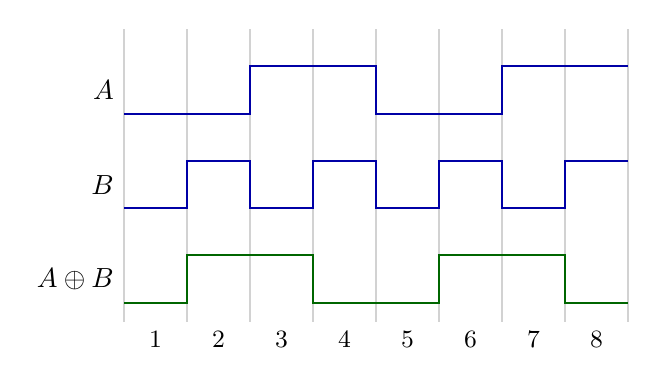
\begin{tikzpicture}[x=8mm,y=6mm,line width=.7pt]
\foreach \x in {0,...,8}{\draw[gray!35] (\x,-.4)--(\x,5.8);}
\node[left] at (0,4.5) {$A$};\node[left] at (0,2.5) {$B$};\node[left] at (0,.5) {$A\oplus B$};
\draw[blue!65!black] (0,4)--(2,4)--(2,5)--(4,5)--(4,4)--(6,4)--(6,5)--(8,5);
\draw[blue!65!black] (0,2)--(1,2)--(1,3)--(2,3)--(2,2)--(3,2)--(3,3)--(4,3)--(4,2)--(5,2)--(5,3)--(6,3)--(6,2)--(7,2)--(7,3)--(8,3);
\draw[green!40!black] (0,0)--(1,0)--(1,1)--(3,1)--(3,0)--(5,0)--(5,1)--(7,1)--(7,0)--(8,0);
\foreach \x in {1,...,8}{\node[below,font=\small] at (\x-.5,-.4) {\x};}
\end{tikzpicture}\end{chThreeDiagram}
\captionof{figure}{প্রতি সময়খণ্ডের ইনপুটে XOR-এর উচ্চ ও নিম্ন output level।}

\end{minipage}
\end{center}
প্রথমে সময়খণ্ডের সীমা নির্ধারণ করে প্রতিটি খণ্ডে সত্যক সারণির নিয়ম বসাও। এই diagram-এ input propagation delay দেখানো হয়নি; বাস্তব গেটে কিছু delay থাকে।

% Mahbub teaching-type follow-up, 2026-10-14
\subsection{একাধিক আউটপুট, সমতুল্য সার্কিট ও পরিবর্তিত গেট}
\chThreeExample{৭}{একই ইনপুট থেকে দুটি output}
তিনটি ইনপুটে $P=AB$, $Y=P+C$ এবং $Z=\overline{P+C}$। সার্কিট ও দুই output-এর সত্যক সারণি দেখাও।
\chThreeAnswer প্রথম AND-এর output P একটি OR-এ C-এর সঙ্গে যায়। OR-এর output সরাসরি Y; ওই output NOT করলে Z।
\begin{center}\begin{minipage}{\linewidth}\centering
\begin{chThreeDiagram}\begin{tikzpicture}[>=Stealth,line width=.7pt]
\node[and gate US,chgate] (a) at (1,1) {};
\node[or gate US,chgate] (o) at (4,.5) {};
\node[not gate US,draw,minimum size=10mm] (n) at (7,-.5) {};
\draw (a.input 1)--++(-.8,0) node[left] {$A$};\draw (a.input 2)--++(-.8,0) node[left] {$B$};
\draw (a.output)--++(.7,0)|-(o.input 1);\draw (o.input 2)--++(-1,0) node[left] {$C$};
\draw[->] (o.output)--(6,.5)--(8,.5) node[right] {$Y$};\fill (6,.5) circle(1.4pt);
\draw (6,.5)|-(n.input);\draw[->] (n.output)--++(.8,0) node[right] {$Z$};
\end{tikzpicture}\end{chThreeDiagram}
\captionof{figure}{একটি intermediate signal থেকে স্বাভাবিক ও পূরক দুই output।}
\end{minipage}\end{center}
\begin{center}\begin{tabular}{|c|c|c|c|c|c|}\hline
$A$&$B$&$C$&$P=AB$&$Y$&$Z$\\\hline
0&0&0&0&0&1\\\hline0&0&1&0&1&0\\\hline0&1&0&0&0&1\\\hline0&1&1&0&1&0\\\hline
1&0&0&0&0&1\\\hline1&0&1&0&1&0\\\hline1&1&0&1&1&0\\\hline1&1&1&1&1&0\\\hline
\end{tabular}\end{center}
সারণিতে input combination একবারই লেখা হয়েছে; আলাদা output-এর জন্য আলাদা column। এখানে প্রতিটি সারিতে $Z=\overline Y$।

\chThreeExample{৮}{সার্কিট সরল করে গেট কমানো}
একটি AND থেকে $P=AB$ পাওয়া যায়; P এবং C দ্বিতীয় AND-এ $Q=PC$ তৈরি করে। শেষ OR-এ P ও Q যায়। সমতুল্য ছোট সার্কিট কী?
\chThreeAnswer $Y=P+Q=AB+ABC=AB(1+C)=AB$। দুটি AND ও একটি OR-এর বদলে একটি AND যথেষ্ট। C আর output নির্ধারণ করে না।
\begin{center}\begin{minipage}{\linewidth}\centering
\begin{chThreeDiagram}\begin{tikzpicture}[>=Stealth,line width=.7pt]
\node[and gate US,chgate] (a) at (0,1) {};
\node[and gate US,chgate] (b) at (2,-.6) {};
\node[or gate US,chgate] (o) at (4,.6) {};
\draw (a.input 1)--++(-.6,0) node[left] {$A$};\draw (a.input 2)--++(-.6,0) node[left] {$B$};
\draw (a.output)--(1,1)--(3,1)|-(o.input 1);\fill (1,1) circle(1.4pt);
\draw (1,1)|-(b.input 1);\draw (b.input 2)--++(-.6,0) node[left] {$C$};\draw (b.output)--++(.4,0)|-(o.input 2);
\draw (o.output)--++(.5,0) node[right] {$Y$};
\node at (6,.6) {$\equiv$};\node[and gate US,chgate] (s) at (8,.6) {};
\draw (s.input 1)--++(-.7,0) node[left] {$A$};\draw (s.input 2)--++(-.7,0) node[left] {$B$};\draw (s.output)--++(.6,0) node[right] {$Y$};
\end{tikzpicture}\end{chThreeDiagram}
\captionof{figure}{অপ্রয়োজনীয় branch বাদ দিয়ে একই কাজের ছোট সার্কিট।}
\end{minipage}\end{center}
দুটি সমীকরণ সমান হলেই তাদের আদর্শ সত্যক সারণি সমান। বাস্তব delay বা বিদ্যুৎ খরচ সমান হওয়ার দাবি এতে করা হয় না।

\chThreeExample{৯}{শেষ গেট বদলালে কোন input-এ ফল বদলায়?}
আগের সার্কিটের শেষ OR-কে AND করো। নতুন output এবং পুরোনোটির সঙ্গে পার্থক্য নির্ণয় করো।
\chThreeAnswer নতুন $Y_1=PQ=(AB)(ABC)=ABC$; পুরোনো $Y=AB$। $A=B=1,C=0$-এ পুরোনো output ১, নতুন output ০। C=১ হলে দুই রাশি সমান; A বা B শূন্য হলেও দুইটিই শূন্য। তাই একমাত্র 110 সারিতে পার্থক্য। একটি নির্দিষ্ট input-এ output মিলে গেলে দুটি circuit-কে সমতুল্য বলা যায় না।

\chThreeExample{১০}{তিন ইনপুটের timing থেকে output}
আট সময়খণ্ডে $A=00001111$, $B=00110011$, $C=01010101$। $Y=(A+B)\overline C$-এর output sequence নির্ণয় করো।
\chThreeAnswer
\begin{center}\begin{tabular}{|l|c|c|c|c|c|c|c|c|}\hline
সময়খণ্ড&১&২&৩&৪&৫&৬&৭&৮\\\hline
$A$&0&0&0&0&1&1&1&1\\\hline
$B$&0&0&1&1&0&0&1&1\\\hline
$C$&0&1&0&1&0&1&0&1\\\hline
$A+B$&0&0&1&1&1&1&1&1\\\hline
$Y$&0&0&1&0&1&0&1&0\\\hline
\end{tabular}\end{center}
ফল 00101010। তৃতীয় খণ্ডে OR-এর মান ১ ও C-এর পূরক ১, তাই Y=১; চতুর্থ খণ্ডে C=১, তাই Y=০। প্রতিটি খণ্ডে intermediate output গণনা করলে বহু গেটের waveform-ও একইভাবে পাওয়া যায়। সময়ক্রমকে এখানে সংখ্যামান হিসেবে পড়ার প্রয়োজন নেই।

\providecommand{\chLogicExample}[3]{\chThreeExample{#2}{#3}\label{ex:#1}}
\subsection{ধরন অনুযায়ী সত্যক সারণি ও circuit বিশ্লেষণ}
প্রতিটি স্বাধীন input-এর combination আগে লেখো। এরপর signal যে ক্রমে gate পেরোয় সেই ক্রমে P,Q ইত্যাদির column পূরণ করো। সারণি থেকে সমীকরণে output ১-এর সারি SOP এবং ০-এর সারি POS-এর জন্য ব্যবহার করা হয়।
\Needspace{12\baselineskip}
\subsubsection*{ধরন ১: সমীকরণ থেকে মধ্যবর্তী column-সহ সত্যক সারণি}
একাধিক operation থাকলে প্রতিটি stage-এর জন্য আলাদা column রাখো। এতে কোথায় পূরক বা AND/OR হয়েছে তা বোঝা যায়।
\par\smallskip\noindent\begin{minipage}{\linewidth}
\chLogicExample{CT01.1}{১.১}{SOP-এর দুই product}
$Y=\overline AB+AC$-এর সত্যক সারণি দাও.
\chThreeAnswer $P=\overline AB$, $Q=AC$; শেষে $Y=P+Q$। A=০ হলে Y=B; A=১ হলে Y=C।
\begin{center}\begin{tabular}{|c|c|c|c|c|c|}\hline
$A$ & $B$ & $C$ & $P$ & $Q$ & $Y$\\\hline
0 & 0 & 0 & 0 & 0 & 0\\\hline
0 & 0 & 1 & 0 & 0 & 0\\\hline
0 & 1 & 0 & 1 & 0 & 1\\\hline
0 & 1 & 1 & 1 & 0 & 1\\\hline
1 & 0 & 0 & 0 & 0 & 0\\\hline
1 & 0 & 1 & 0 & 1 & 1\\\hline
1 & 1 & 0 & 0 & 0 & 0\\\hline
1 & 1 & 1 & 0 & 1 & 1\\\hline
\end{tabular}\end{center}

\end{minipage}\par\smallskip
\par\smallskip\noindent\begin{minipage}{\linewidth}
\chLogicExample{CT01.2}{১.২}{POS-এর দুই sum}
$Y=(A+B)(\overline B+C)$-এর সারণি দাও.
\chThreeAnswer $P=A+B$, $Q=\overline B+C$; Y=PQ। B=০ হলে Y=A; B=১ হলে Y=C।
\begin{center}\begin{tabular}{|c|c|c|c|c|c|}\hline
$A$ & $B$ & $C$ & $P$ & $Q$ & $Y$\\\hline
0 & 0 & 0 & 0 & 1 & 0\\\hline
0 & 0 & 1 & 0 & 1 & 0\\\hline
0 & 1 & 0 & 1 & 0 & 0\\\hline
0 & 1 & 1 & 1 & 1 & 1\\\hline
1 & 0 & 0 & 1 & 1 & 1\\\hline
1 & 0 & 1 & 1 & 1 & 1\\\hline
1 & 1 & 0 & 1 & 0 & 0\\\hline
1 & 1 & 1 & 1 & 1 & 1\\\hline
\end{tabular}\end{center}

\end{minipage}\par\smallskip
\Needspace{12\baselineskip}
\subsubsection*{ধরন ২: সত্যক সারণি থেকে SOP ও POS}
১-এর সারিতে input ০ হলে চলকের পূরক দিয়ে AND পদ বানাও। ০-এর সারিতে input ১ হলে পূরক দিয়ে OR পদ বানাও। সব চলক না থাকলে পদটি canonical minterm/maxterm নয়।
\par\smallskip\noindent\begin{minipage}{\linewidth}
\chLogicExample{CT02.1}{২.১}{দুই চলকের নির্দিষ্ট দুই সারি}
00,01,10,11 ক্রমে Y=0101। SOP এবং POS নির্ণয় করো.
\chThreeAnswer ১-এর সারি 01,11: $Y=\overline AB+AB=B$। ০-এর সারি 00,10: $Y=(A+B)(\overline A+B)=B$। A ফল নির্ধারণ করে না।
\begin{center}\begin{tabular}{|c|c|c|}\hline
$A$ & $B$ & $Y$\\\hline
0 & 0 & 0\\\hline
0 & 1 & 1\\\hline
1 & 0 & 0\\\hline
1 & 1 & 1\\\hline
\end{tabular}\end{center}

\end{minipage}\par\smallskip
\par\smallskip\noindent\begin{minipage}{\linewidth}
\chLogicExample{CT02.2}{২.২}{চার চলকের ১৬ সারি}
A,B,C,D ক্রমে শুধু 0011,0111,1011,1111-তে Y=১। সমীকরণ নির্ণয় করো.
\chThreeAnswer $Y=\overline A\,\overline BCD+\overline ABCD+A\overline BCD+ABCD=CD(\overline A+A)(\overline B+B)=CD$। চার independent input থাকায় সারণিতে ১৬ সারি, output রাশিতে পরে দুই চলক থাকলেও।
\begin{center}\begin{tabular}{|c|c|c|c|c|}\hline
$A$ & $B$ & $C$ & $D$ & $Y$\\\hline
0 & 0 & 0 & 0 & 0\\\hline
0 & 0 & 0 & 1 & 0\\\hline
0 & 0 & 1 & 0 & 0\\\hline
0 & 0 & 1 & 1 & 1\\\hline
0 & 1 & 0 & 0 & 0\\\hline
0 & 1 & 0 & 1 & 0\\\hline
0 & 1 & 1 & 0 & 0\\\hline
0 & 1 & 1 & 1 & 1\\\hline
1 & 0 & 0 & 0 & 0\\\hline
1 & 0 & 0 & 1 & 0\\\hline
1 & 0 & 1 & 0 & 0\\\hline
1 & 0 & 1 & 1 & 1\\\hline
1 & 1 & 0 & 0 & 0\\\hline
1 & 1 & 0 & 1 & 0\\\hline
1 & 1 & 1 & 0 & 0\\\hline
1 & 1 & 1 & 1 & 1\\\hline
\end{tabular}\end{center}

\end{minipage}\par\smallskip
\Needspace{12\baselineskip}
\subsubsection*{ধরন ৩: diagram থেকে equation ও নির্দিষ্ট output}
প্রথম gate থেকে শেষ gate পর্যন্ত P,Q,R লিখে এগোও। output bubble থাকলে পুরো gate-এর ফলের পূরক নাও।
\par\smallskip\noindent\begin{minipage}{\linewidth}
\chLogicExample{CT03.1}{৩.১}{NAND ও NOR-এর যৌগিক circuit}
চিত্রের Y-এর সমীকরণ লেখো এবং A=১,B=০,C=১-এ output বের করো.
\chThreeAnswer $P=\overline{AB}$, $Q=\overline{P+C}$, $Y=\overline Q$। তাই $Y=P+C=\overline{AB}+C$। দেওয়া input-এ P=১,Q=০,Y=১।
\begin{center}\begin{minipage}{\linewidth}\centering
\begin{chThreeDiagram}\begin{tikzpicture}[>=Stealth,line width=.85pt,draw=ICTBlue,font=\small]
\node[nand gate US,draw,fill=ICTLightBlue,logic gate inputs=nn,minimum size=10mm] (P) at (0,0.6) {};
\node[nor gate US,draw,fill=ICTLightBlue,logic gate inputs=nn,minimum size=10mm] (Q) at (3,0) {};
\node[not gate US,draw,fill=ICTLightBlue,logic gate inputs=n,minimum size=10mm] (Y) at (6,0) {};
\draw (P.input 1)--++(-.7,0) node[left,text=black] {$A$};
\draw (P.input 2)--++(-.7,0) node[left,text=black] {$B$};
\node[above=3pt,text=ICTGreen] at (P.north) {$P$};
\draw (P.output)--(0.85,0.6) |- (Q.input 1);
\draw (Q.input 2)--++(-.7,0) node[left,text=black] {$C$};
\node[above=3pt,text=ICTGreen] at (Q.north) {$Q$};
\draw (Q.output)--(3.85,0) |- (Y.input);
\draw[->] (Y.output)--++(.85,0) node[right,text=black] {$Y$};
\end{tikzpicture}\end{chThreeDiagram}
\captionof{figure}{তিন stage-এর output ও পূরকের সীমা।}\label{LG014}
\end{minipage}\end{center}

\end{minipage}\par\smallskip
\par\smallskip\noindent\begin{minipage}{\linewidth}
\chLogicExample{CT03.2}{৩.২}{দুটি output-এর পৃথক পথ}
চিত্রে $P=A\oplus B$, $Y=PC$, $Z=\overline{P+C}$। A=১,B=০,C=১-এ Y,Z কত?
\chThreeAnswer P=১, তাই Y=১ ও Z=০। Y-তে AND, Z-তে NOR; একই P থেকে বেরোলেও output দুটির নিয়ম আলাদা।
\begin{center}\begin{minipage}{\linewidth}\centering
\begin{chThreeDiagram}\begin{tikzpicture}[>=Stealth,line width=.85pt,draw=ICTBlue,font=\small]
\node[xor gate US,draw,fill=ICTLightBlue,logic gate inputs=nn,minimum size=10mm] (P) at (0,0) {};
\node[and gate US,draw,fill=ICTLightBlue,logic gate inputs=nn,minimum size=10mm] (Y) at (3,1.2) {};
\node[nor gate US,draw,fill=ICTLightBlue,logic gate inputs=nn,minimum size=10mm] (Z) at (3,-1.2) {};
\draw (P.input 1)--++(-.7,0) node[left,text=black] {$A$};
\draw (P.input 2)--++(-.7,0) node[left,text=black] {$B$};
\node[above=3pt,text=ICTGreen] at (P.north) {$P$};
\fill[ICTBlue] (0.85,0) circle (1.2pt);
\draw (P.output)--(0.85,0) |- (Y.input 1);
\draw (Y.input 2)--++(-.7,0) node[left,text=black] {$C$};
\draw (P.output)--(0.85,0) |- (Z.input 1);
\draw (Z.input 2)--++(-.7,0) node[left,text=black] {$C$};
\draw[->] (Y.output)--++(.85,0) node[right,text=black] {$Y$};
\draw[->] (Z.output)--++(.85,0) node[right,text=black] {$Z$};
\end{tikzpicture}\end{chThreeDiagram}
\captionof{figure}{এক intermediate থেকে দুই পৃথক output branch।}\label{LG015}
\end{minipage}\end{center}

\end{minipage}\par\smallskip
\Needspace{12\baselineskip}
\subsubsection*{ধরন ৪: রাশি থেকে মৌলিক gate-এর circuit}
NOT দিয়ে প্রয়োজনীয় পূরক তৈরি করো। AND/OR-এর বন্ধনী এবং gate-এর input সংখ্যা মেলাও; circuit-এর output equation দিয়ে আবার পরীক্ষা করো।
\par\smallskip\noindent\begin{minipage}{\linewidth}
\chLogicExample{CT04.1}{৪.১}{দুটি AND পরে OR}
$Y=A\overline B+C\overline D$-এর মৌলিক gate circuit আঁকো.
\chThreeAnswer $N_B=\overline B$, $N_D=\overline D$; $P=AN_B$, $Q=CN_D$; $Y=P+Q$। দুই NOT, দুই AND ও এক OR।
\begin{center}\begin{minipage}{\linewidth}\centering
\begin{chThreeDiagram}\begin{tikzpicture}[>=Stealth,line width=.85pt,draw=ICTBlue,font=\small]
\node[not gate US,draw,fill=ICTLightBlue,logic gate inputs=n,minimum size=10mm] (NB) at (0,1.2) {};
\node[not gate US,draw,fill=ICTLightBlue,logic gate inputs=n,minimum size=10mm] (ND) at (0,-1.2) {};
\node[and gate US,draw,fill=ICTLightBlue,logic gate inputs=nn,minimum size=10mm] (P) at (3,1.2) {};
\node[and gate US,draw,fill=ICTLightBlue,logic gate inputs=nn,minimum size=10mm] (Q) at (3,-1.2) {};
\node[or gate US,draw,fill=ICTLightBlue,logic gate inputs=nn,minimum size=10mm] (Y) at (6,0) {};
\draw (NB.input)--++(-.7,0) node[left,text=black] {$B$};
\node[above=3pt,text=ICTGreen] at (NB.north) {$N_B$};
\draw (ND.input)--++(-.7,0) node[left,text=black] {$D$};
\node[above=3pt,text=ICTGreen] at (ND.north) {$N_D$};
\draw (P.input 1)--++(-.7,0) node[left,text=black] {$A$};
\draw (NB.output)--(0.97,1.2) |- (P.input 2);
\node[above=3pt,text=ICTGreen] at (P.north) {$P$};
\draw (Q.input 1)--++(-.7,0) node[left,text=black] {$C$};
\draw (ND.output)--(0.97,-1.2) |- (Q.input 2);
\node[above=3pt,text=ICTGreen] at (Q.north) {$Q$};
\draw (P.output)--(3.85,1.2) |- (Y.input 1);
\draw (Q.output)--(3.97,-1.2) |- (Y.input 2);
\draw[->] (Y.output)--++(.85,0) node[right,text=black] {$Y$};
\end{tikzpicture}\end{chThreeDiagram}
\captionof{figure}{মৌলিক gate-এ চার-input SOP।}\label{LG016}
\end{minipage}\end{center}

\end{minipage}\par\smallskip
\par\smallskip\noindent\begin{minipage}{\linewidth}
\chLogicExample{CT04.2}{৪.২}{দুটি OR পরে AND}
$Y=(A+\overline C)(B+D)$-এর circuit আঁকো.
\chThreeAnswer $N_C=\overline C$, $P=A+N_C$, $Q=B+D$, $Y=PQ$। এক NOT, দুই OR ও এক AND।
\begin{center}\begin{minipage}{\linewidth}\centering
\begin{chThreeDiagram}\begin{tikzpicture}[>=Stealth,line width=.85pt,draw=ICTBlue,font=\small]
\node[not gate US,draw,fill=ICTLightBlue,logic gate inputs=n,minimum size=10mm] (NC) at (0,1.2) {};
\node[or gate US,draw,fill=ICTLightBlue,logic gate inputs=nn,minimum size=10mm] (P) at (3,1.2) {};
\node[or gate US,draw,fill=ICTLightBlue,logic gate inputs=nn,minimum size=10mm] (Q) at (3,-1.2) {};
\node[and gate US,draw,fill=ICTLightBlue,logic gate inputs=nn,minimum size=10mm] (Y) at (6,0) {};
\draw (NC.input)--++(-.7,0) node[left,text=black] {$C$};
\node[above=3pt,text=ICTGreen] at (NC.north) {$N_C$};
\draw (P.input 1)--++(-.7,0) node[left,text=black] {$A$};
\draw (NC.output)--(0.97,1.2) |- (P.input 2);
\node[above=3pt,text=ICTGreen] at (P.north) {$P$};
\draw (Q.input 1)--++(-.7,0) node[left,text=black] {$B$};
\draw (Q.input 2)--++(-.7,0) node[left,text=black] {$D$};
\node[above=3pt,text=ICTGreen] at (Q.north) {$Q$};
\draw (P.output)--(3.85,1.2) |- (Y.input 1);
\draw (Q.output)--(3.97,-1.2) |- (Y.input 2);
\draw[->] (Y.output)--++(.85,0) node[right,text=black] {$Y$};
\end{tikzpicture}\end{chThreeDiagram}
\captionof{figure}{মৌলিক gate-এ চার-input POS।}\label{LG017}
\end{minipage}\end{center}

\end{minipage}\par\smallskip
\Needspace{12\baselineskip}
\subsubsection*{ধরন ৫: সরলীকরণ ও gate পরিবর্তনের তুলনা}
আগের ও পরের সমীকরণ পাশাপাশি লিখে সত্যক সারণিতে তুলনা করো। gate কমানো এবং gate-এর ধরন বদলানো সবসময় একই ফল দেয় না।
\par\smallskip\noindent\begin{minipage}{\linewidth}
\chLogicExample{CT05.1}{৫.১}{অপ্রয়োজনীয় branch বাদ}
$P=AC$, $Q=PB$, $Y=P+Q$। ছোট circuit দাও.
\chThreeAnswer $Y=AC+ABC=AC$। আগে দুই AND ও এক OR; পরে এক AND। B বাদ পড়ে। A=C=১ হলেই Y=১।
\begin{center}\begin{minipage}{\linewidth}\centering
\begin{chThreeDiagram}\begin{tikzpicture}[>=Stealth,line width=.85pt,draw=ICTBlue,font=\small]
\node[and gate US,draw,fill=ICTLightBlue,logic gate inputs=nn,minimum size=10mm] (Y) at (0,0) {};
\draw (Y.input 1)--++(-.7,0) node[left,text=black] {$A$};
\draw (Y.input 2)--++(-.7,0) node[left,text=black] {$C$};
\draw[->] (Y.output)--++(.85,0) node[right,text=black] {$Y$};
\end{tikzpicture}\end{chThreeDiagram}
\captionof{figure}{Absorption-এর পরে এক AND-এর সমতুল্য circuit।}\label{LG018}
\end{minipage}\end{center}

\end{minipage}\par\smallskip
\par\smallskip\noindent\begin{minipage}{\linewidth}
\chLogicExample{CT05.2}{৫.২}{শেষ gate OR থেকে XOR}
$P=AB$, $Q=AC$। পুরোনো Y=P+Q; নতুন Z=P\oplus Q। কখন ফল বদলাবে?
\chThreeAnswer P=Q=১ হলে OR দেয় ১, XOR দেয় ০। অর্থাৎ A=B=C=১-এ পার্থক্য। অন্য সাত সারিতে একই ফল। শেষ gate বদলানোর আগে 111 সারিও পরীক্ষা করতে হবে।
\begin{center}\begin{tabular}{|c|c|c|c|c|c|c|}\hline
$A$ & $B$ & $C$ & $P$ & $Q$ & $Y$ & $Z$\\\hline
0 & 0 & 0 & 0 & 0 & 0 & 0\\\hline
0 & 0 & 1 & 0 & 0 & 0 & 0\\\hline
0 & 1 & 0 & 0 & 0 & 0 & 0\\\hline
0 & 1 & 1 & 0 & 0 & 0 & 0\\\hline
1 & 0 & 0 & 0 & 0 & 0 & 0\\\hline
1 & 0 & 1 & 0 & 1 & 1 & 1\\\hline
1 & 1 & 0 & 1 & 0 & 1 & 1\\\hline
1 & 1 & 1 & 1 & 1 & 1 & 0\\\hline
\end{tabular}\end{center}

\end{minipage}\par\smallskip
\Needspace{12\baselineskip}
\subsubsection*{ধরন ৬: timing diagram থেকে output sequence}
সময়ের প্রতিটি খণ্ডে input স্থির ধরে gate-এর নিয়ম বসাও। এখানে ideal gate; propagation delay উপেক্ষা করা হয়েছে। waveform একটি সময়ক্রম, সবসময় সংখ্যামান নয়।
\par\smallskip\noindent\begin{minipage}{\linewidth}
\chLogicExample{CT06.1}{৬.১}{দুই gate-এর waveform}
আট সময়খণ্ডে A=01011010, B=00110101। XOR ও NOR-এর waveform আঁকো।
\chThreeAnswer XOR-এর P=01101111; NOR-এর Y=10000000। প্রতি column-এ ভিন্ন input হলে P=১ এবং দুই input-ই ০ হলে Y=১।
\begin{center}\begin{tabular}{|c|c|c|c|c|c|c|c|c|}\hline
সময়খণ্ড & ১ & ২ & ৩ & ৪ & ৫ & ৬ & ৭ & ৮\\\hline
$A$ & 0 & 1 & 0 & 1 & 1 & 0 & 1 & 0\\\hline
$B$ & 0 & 0 & 1 & 1 & 0 & 1 & 0 & 1\\\hline
$P=A\oplus B$ & 0 & 1 & 1 & 0 & 1 & 1 & 1 & 1\\\hline
$Y=\overline{A+B}$ & 1 & 0 & 0 & 0 & 0 & 0 & 0 & 0\\\hline
\end{tabular}\end{center}
\begin{center}\begin{minipage}{\linewidth}\centering\begin{chThreeDiagram}\begin{tikzpicture}[x=9mm,y=5mm,line width=.85pt]
\draw[gray!25] (0,-.7)--(0,11.5);
\draw[gray!25] (1,-.7)--(1,11.5);
\draw[gray!25] (2,-.7)--(2,11.5);
\draw[gray!25] (3,-.7)--(3,11.5);
\draw[gray!25] (4,-.7)--(4,11.5);
\draw[gray!25] (5,-.7)--(5,11.5);
\draw[gray!25] (6,-.7)--(6,11.5);
\draw[gray!25] (7,-.7)--(7,11.5);
\draw[gray!25] (8,-.7)--(8,11.5);
\node[left] at (0,9.5) {$A$};
\draw[ICTBlue] (0,9)--(1,9)--(1,10)--(2,10)--(2,9)--(3,9)--(3,10)--(4,10)--(4,10)--(5,10)--(5,9)--(6,9)--(6,10)--(7,10)--(7,9)--(8,9);
\node[left] at (0,6.5) {$B$};
\draw[ICTBlue] (0,6)--(1,6)--(1,6)--(2,6)--(2,7)--(3,7)--(3,7)--(4,7)--(4,6)--(5,6)--(5,7)--(6,7)--(6,6)--(7,6)--(7,7)--(8,7);
\node[left] at (0,3.5) {$P$};
\draw[ICTBlue] (0,3)--(1,3)--(1,4)--(2,4)--(2,4)--(3,4)--(3,3)--(4,3)--(4,4)--(5,4)--(5,4)--(6,4)--(6,4)--(7,4)--(7,4)--(8,4);
\node[left] at (0,0.5) {$Y$};
\draw[ICTBlue] (0,1)--(1,1)--(1,0)--(2,0)--(2,0)--(3,0)--(3,0)--(4,0)--(4,0)--(5,0)--(5,0)--(6,0)--(6,0)--(7,0)--(7,0)--(8,0);
\node[below] at (0.5,-.6) {১};
\node[below] at (1.5,-.6) {২};
\node[below] at (2.5,-.6) {৩};
\node[below] at (3.5,-.6) {৪};
\node[below] at (4.5,-.6) {৫};
\node[below] at (5.5,-.6) {৬};
\node[below] at (6.5,-.6) {৭};
\node[below] at (7.5,-.6) {৮};
\end{tikzpicture}\end{chThreeDiagram}
\captionof{figure}{XOR ও NOR-এর আট সময়খণ্ডের output।}\label{LG019}
\end{minipage}\end{center}
\end{minipage}\par\smallskip
\par\smallskip\noindent\begin{minipage}{\linewidth}
\chLogicExample{CT06.2}{৬.২}{দুই gate-এর waveform}
আট সময়খণ্ডে A=11100010, B=01010110। XOR ও NOR-এর waveform আঁকো।
\chThreeAnswer XOR-এর P=10110100; NOR-এর Y=00001001। প্রতি column-এ ভিন্ন input হলে P=১ এবং দুই input-ই ০ হলে Y=১।
\begin{center}\begin{tabular}{|c|c|c|c|c|c|c|c|c|}\hline
সময়খণ্ড & ১ & ২ & ৩ & ৪ & ৫ & ৬ & ৭ & ৮\\\hline
$A$ & 1 & 1 & 1 & 0 & 0 & 0 & 1 & 0\\\hline
$B$ & 0 & 1 & 0 & 1 & 0 & 1 & 1 & 0\\\hline
$P=A\oplus B$ & 1 & 0 & 1 & 1 & 0 & 1 & 0 & 0\\\hline
$Y=\overline{A+B}$ & 0 & 0 & 0 & 0 & 1 & 0 & 0 & 1\\\hline
\end{tabular}\end{center}
\begin{center}\begin{minipage}{\linewidth}\centering\begin{chThreeDiagram}\begin{tikzpicture}[x=9mm,y=5mm,line width=.85pt]
\draw[gray!25] (0,-.7)--(0,11.5);
\draw[gray!25] (1,-.7)--(1,11.5);
\draw[gray!25] (2,-.7)--(2,11.5);
\draw[gray!25] (3,-.7)--(3,11.5);
\draw[gray!25] (4,-.7)--(4,11.5);
\draw[gray!25] (5,-.7)--(5,11.5);
\draw[gray!25] (6,-.7)--(6,11.5);
\draw[gray!25] (7,-.7)--(7,11.5);
\draw[gray!25] (8,-.7)--(8,11.5);
\node[left] at (0,9.5) {$A$};
\draw[ICTBlue] (0,10)--(1,10)--(1,10)--(2,10)--(2,10)--(3,10)--(3,9)--(4,9)--(4,9)--(5,9)--(5,9)--(6,9)--(6,10)--(7,10)--(7,9)--(8,9);
\node[left] at (0,6.5) {$B$};
\draw[ICTBlue] (0,6)--(1,6)--(1,7)--(2,7)--(2,6)--(3,6)--(3,7)--(4,7)--(4,6)--(5,6)--(5,7)--(6,7)--(6,7)--(7,7)--(7,6)--(8,6);
\node[left] at (0,3.5) {$P$};
\draw[ICTBlue] (0,4)--(1,4)--(1,3)--(2,3)--(2,4)--(3,4)--(3,4)--(4,4)--(4,3)--(5,3)--(5,4)--(6,4)--(6,3)--(7,3)--(7,3)--(8,3);
\node[left] at (0,0.5) {$Y$};
\draw[ICTBlue] (0,0)--(1,0)--(1,0)--(2,0)--(2,0)--(3,0)--(3,0)--(4,0)--(4,1)--(5,1)--(5,0)--(6,0)--(6,0)--(7,0)--(7,1)--(8,1);
\node[below] at (0.5,-.6) {১};
\node[below] at (1.5,-.6) {২};
\node[below] at (2.5,-.6) {৩};
\node[below] at (3.5,-.6) {৪};
\node[below] at (4.5,-.6) {৫};
\node[below] at (5.5,-.6) {৬};
\node[below] at (6.5,-.6) {৭};
\node[below] at (7.5,-.6) {৮};
\end{tikzpicture}\end{chThreeDiagram}
\captionof{figure}{XOR ও NOR-এর আট সময়খণ্ডের output।}\label{LG020}
\end{minipage}\end{center}
\end{minipage}\par\smallskip

